\documentclass[reprint,english,notitlepage]{revtex4-1}  % defines the basic parameters of the document

% if you want a single-column, remove reprint

% allows special characters (including æøå)
\usepackage[utf8]{inputenc}
\usepackage[english]{babel}

%% note that you may need to download some of these packages manually, it depends on your setup.
%% I recommend downloading TeXMaker, because it includes a large library of the most common packages.

\usepackage{physics,amssymb}  % mathematical symbols (physics imports amsmath)
\usepackage{graphicx}         % include graphics such as plots
\graphicspath{{figs/}} %Setting the graphicspath
\numberwithin{equation}{section}
\def\thesection{\arabic{section}}

\usepackage{xcolor}           % set colors
\usepackage{hyperref}         % automagic cross-referencing (this is GODLIKE)
\usepackage{tikz}             % draw figures manually
\usepackage{listings}         % display code
\usepackage{subfigure}        % imports a lot of cool and useful figure commands
\usepackage{pythonhighlight}

% defines the color of hyperref objects
% Blending two colors:  blue!80!black  =  80% blue and 20% black
\hypersetup{ % this is just my personal choice, feel free to change things
    colorlinks,
    linkcolor={red!50!black},
    citecolor={blue!50!black},
    urlcolor={blue!80!black}}

%% Defines the style of the programming listing
%% This is actually my personal template, go ahead and change stuff if you want
\lstset{ %
	inputpath=,
	backgroundcolor=\color{white!88!black},
	basicstyle={\ttfamily\scriptsize},
	commentstyle=\color{magenta},
	language=Python,
	morekeywords={True,False},
	tabsize=4,
	stringstyle=\color{green!55!black},
	frame=single,
	keywordstyle=\color{blue},
	showstringspaces=false,
	columns=fullflexible,
	keepspaces=true}


%% USEFUL LINKS:
%%
%%   UiO LaTeX guides:        https://www.mn.uio.no/ifi/tjenester/it/hjelp/latex/
%%   mathematics:             https://en.wikibooks.org/wiki/LaTeX/Mathematics

%%   PHYSICS !                https://mirror.hmc.edu/ctan/macros/latex/contrib/physics/physics.pdf

%%   the basics of Tikz:       https://en.wikibooks.org/wiki/LaTeX/PGF/TikZ
%%   all the colors!:          https://en.wikibooks.org/wiki/LaTeX/Colors
%%   how to draw tables:       https://en.wikibooks.org/wiki/LaTeX/Tables
%%   code listing styles:      https://en.wikibooks.org/wiki/LaTeX/Source_Code_Listings
%%   \includegraphics          https://en.wikibooks.org/wiki/LaTeX/Importing_Graphics
%%   learn more about figures  https://en.wikibooks.org/wiki/LaTeX/Floats,_Figures_and_Captions
%%   automagic bibliography:   https://en.wikibooks.org/wiki/LaTeX/Bibliography_Management  (this one is kinda difficult the first time)
%%   REVTeX Guide:             http://www.physics.csbsju.edu/370/papers/Journal_Style_Manuals/auguide4-1.pdf
%%
%%   (this document is of class "revtex4-1", the REVTeX Guide explains how the class works)


%% CREATING THE .pdf FILE USING LINUX IN THE TERMINAL
%%
%% [terminal]$ pdflatex template.tex
%%
%% Run the command twice, always.
%% If you want to use \footnote, you need to run these commands (IN THIS SPECIFIC ORDER)
%%
%% [terminal]$ pdflatex template.tex
%% [terminal]$ bibtex template
%% [terminal]$ pdflatex template.tex
%% [terminal]$ pdflatex template.tex
%%
%% Don't ask me why, I don't know.

\begin{document}
\title{AST3220 - Project 2: \\ Big Bang Nuclesynthesis}   % self-explanatory
\author{Candidate nr. 14}
\date{\today}                             % self-explanatory
\noaffiliation                            % ignore this
               % marks the end of the abstract
\maketitle                                % creates the title, author, date & abstract

% the fundamental components of scientific reports:
\section{Problem a)}
 We can rewrite the number density $n_i$ of species $i$ in terms of the relative number
 density $Y_i$ as:
\begin{align}
	Y_i = \frac{n_i}{n_b} \ \ \Rightarrow \ \ n_i &= n_b Y_i \label{eq:rel_no_density} \\
																						&= \frac{n_{b0}}{a^3}Y_i
\end{align}
Where $n_b(t)$ is the baryon number density, $n_{b0}$ is the baryon number
density today, and $a(t)$ is the scale factor. Using the product rule for
differentiation, we can then write
\begin{align}
	\frac{d n_i}{dt} &= n_{b0}\frac{d}{dt}\left(Y_i a^{-3}\right) \\
									 &= n_{b0}\left(\frac{1}{a^3}\frac{dY_i}{dt} - 3Y_i\frac{\dot{a}}{a^4}\right) \\
									 &= n_b \frac{dY_i}{dt} - 3 Y_i n_b H \label{eq:no_density} \\
									 &= n_b \frac{dY_i}{dt} - 3 n_i H \label{eq:no_density}
\end{align}
Next we want to switch from $t$ to $\ln T$ as our time variable, where
$T$ is the temperature. Using $T=T_0 a^{-1}$ we get
\begin{align}
	\ln T = \ln T_0 - \ln a(t)
\end{align}
Then, using the chain rule of differentiation, we can rewrite
\begin{align}
	\frac{dY_i}{dt} &= \frac{d(\ln T)}{dt} \frac{dY_i}{d(\ln T)} \\
									&= -\frac{\dot{a}}{a} \frac{dY_i}{d(\ln T)} \\
									&= -H \frac{dY_i}{d(\ln T)}
\end{align}
Inserting to equation (\ref{eq:no_density}) we get
\begin{align}
	\frac{d n_i}{dt} &= - n_b H \frac{dY_i}{d(\ln T)} - 3 n_i H \label{eq:dndt}
\end{align}
The equations for the evolution of the number densities of protons $p$ and
neutrons $n$ are given as
\begin{align}
	\frac{d n_n}{dt} + 3H n_n &= n_p \Gamma_{p\rightarrow n} - n_n\Gamma_{n\rightarrow p} \\
	\frac{d n_p}{dt} + 3H n_p &= n_n\Gamma_{n\rightarrow p} - n_p \Gamma_{p\rightarrow n}  \\
														&= - \left( \frac{d n_n}{dt} + 3H n_n \right)
\end{align}
Inserting equation \ref{eq:dndt} into these, we get
\begin{align}
	-n_b H \frac{dY_n}{d(\ln T)} = n_p \Gamma_{p\rightarrow n} - n_n \Gamma_{n\rightarrow p} \\
	-n_b H \frac{dY_p}{d(\ln T)} = n_n \Gamma_{n\rightarrow p} - n_p \Gamma_{p\rightarrow n}
\end{align}
Dividing by $-n_b H$ and using Eq. (\ref{eq:rel_no_density}) we finally get:
\begin{align}
	\frac{dY_n}{d(\ln T)} = -\frac{1}{H}\left[Y_p\Gamma_{p\rightarrow n} - Y_n \Gamma_{n\rightarrow p}\right] \\
	\frac{dY_p}{d(\ln T)} = -\frac{1}{H}\left[Y_n\Gamma_{n\rightarrow p} - Y_p \Gamma_{p\rightarrow n}\right]
\end{align}
\section{Problem b)}
The relation $T_\nu = \left(4/11)^{1/3} T$ can be derived from the conservation
of entropy, which tells us that
\begin{align}
	g_{*s}(aT)^3 = const.
\end{align}
At the time where the universe had a temperature $k_B T > 0.511$ Mev, electrons
and positrons were relativistic and the process
\begin{align}
	e^+ + e^- \rightleftharpoons \gamma + \gamma
\end{align}
occured in both directions. However, as the temperature universe falls below the
rest mass of the electron and positron $k_B T < 0.511$, the average energy of a
photon collision is too small for an electrons-positron pair to be created.
Since electrons and positrons will still anihilate through the process
\begin{align}
	e^+ + e^- \rightarrow \gamma + \gamma
\end{align}
and most of the positrons and electrons will then dissapear. Assuming this happened
immediately, and that the universe is in thermal equilibrium ($T_i=T$), the
effective number of degrees of freedom before and after can be written
\begin{align}
	g_{*s}^\mathrm{before} &= g_\nu + \frac{7}{8}(g_{e^-} + g_{e^+}) \\
									&= 2 + \frac{7}{8}4 \\
									&= \frac{11}{2} \\
	g_{*s}^\mathrm{after} &= g_\nu \\
								 &= 2
\end{align}
If we also assume the scale factor $a$ is the same before and after, the
conservation of entropy gives us
\begin{align}
	\frac{11}{2}(aT)_\mathrm{before}^3 = 2(aT)_\mathrm{after}^3 \\
	\Rightarrow T_\mathrm{after} = (\frac{11}{4})^{1/3} T_\mathrm{before}
\end{align}
Assuming neutrinos were already decoupled before this time, the neutrino temperature
would remain unaffected:
\begin{align}
	T_{\nu,\mathrm{after}} = T_{\nu,\mathrm{before}}
\end{align}
If we then choose $T_{\nu,\mathrm{before}}$ to be some time before neutrino decoupling,
we expect neutrinos and photons to be in a state of thermal equilibrium,
such that the neutron temperature and photon temperature are equal
\begin{align}
	T_{\nu,\mathrm{before}} = T_\mathrm{before}
\end{align}
We then find that
\begin{align}
	T_{\nu,\mathrm{after}} = T_{\nu,\mathrm{before}} = T_\mathrm{before} = \left(\frac{4}{11}\right)^{1/3} \ T_\mathrm{after}
\end{align}
Finally giving us an expression for the neutrino temperature today
\begin{align}
	T_\nu = \left(\frac{4}{11}\right)^{1/3} \ T
\end{align}
Where we have renamed $T_{\nu,\mathrm{after}} = T_{\nu,\mathrm{before}} = T_\nu$, as well as
$T_\mathrm{after} = T$.
\section{Problem c)}
In the early universe, dominated by radiation, we have
\begin{align}
	\rho c^2 \approx \frac{\pi^2}{30} g_* \frac{(k_b T)^4}{(\hbar c)^3}
\end{align}
Where $g_*$ is the effective number of relativistic degrees of freedom. Assuming
all the radiation is composed of photons and $N_\mathrm{eff}$ number of neutrino species,
$g_*$ is
\begin{align}
	g_* &= 1 + N_{\mathrm{eff}}\ g_\nu	\left( \frac{T_i}{T} \right)^4 \\ %\Sum\limits_{i=\mathrm{bosons}}g_i\frac{}{}
	    &= 1 + N_{\mathrm{eff}}\ \frac{7}{8}	\left(\frac{4}{11}\right)^{4/3}
\end{align}
With $\rho_{c0}=\frac{3H_0^2}{8\pi G}$ as the critical density, we then find
\begin{align}
	\Omega_{r0} &= \frac{\rho_{0}}{\rho_{c0}} \\
							&= \frac{1}{c^2} \left(\frac{\pi^2}{30} g_*
								\frac{(k_b T)^4}{(\hbar c)^3  }\right)\cdot
								\left({\frac{8\pi G}{3H_0^2}}\right) \\
							&= \frac{4\pi^3}{45}\frac{G}{H_0^2}\frac{(k_b T_0)^4}{\hbar^3 c^5}
								g_* \\
							&= \frac{4\pi^3}{45}\frac{G}{H_0^2}\frac{(k_b T_0)^4}{\hbar^3 c^5}
								\left[1 + N_{\mathrm{eff}}\ \frac{7}{8}	\left(\frac{4}{11}\right)^{4/3}\right]
\end{align}
\section{Problem d)}
\subsubsection{Scale factor}
At the time of the BBN, the Friedmann equations simplify to
\begin{align}
	\frac{1}{a} \frac{da}{dt} = \frac{1}{a^2}H_0 \sqrt{\Omega_{r0}}
\end{align}
With some rearranging we see this is a separable differential equation, which
we solve for $a(t)$:
\begin{align}
					 			 a\ \frac{da}{dt} &= H_0 \sqrt{\Omega_{r0}}\ \\
	\Rightarrow\ \ \int_0^a a'\ da' &= H_0 \sqrt{\Omega_{r0}} \int_0^t dt' \\
	\Rightarrow\ \   \frac{1}{2}a^2 &= H_0\sqrt{\Omega_{r0}}t \\
	\Rightarrow\ \ 	  				    a &= \sqrt{2 H_0 t}\  \left(\Omega_{r0}\right)^{1/4}
	\label{eq:a(t)}
\end{align}

\subsubsection{Cosmic time}
To find the cosmic time as a function of the photon temperature, we use the
relation
\begin{align}
	T = T_0 a^{-1} \ \ \Rightarrow \ \ a = \frac{T_0}{T}
\end{align}
Inserting this into equation (\ref{eq:a(t)}) and squaring both sides we get
\begin{align}
	\left(\frac{T_0}{T}\right)^2 &= 2 H_0 t \sqrt{(\Omega_{r0})} \\
\end{align}
Which is easily solved:
\begin{align}
	t(T) = \frac{1}{2 H_0 \sqrt{\Omega_{r0}}} \left(\frac{T_0}{T}\right)^2
\end{align}
A table of this expression evaluated at temperatures $10^{10}$, $10^9$ and $10^8$
is attached in table (\ref{tab:t(T)})

\begin{table}[h!]
	\begin{tabular}{lr}
	\hline
	      $T$ [K] &   $t(T)$ \\
	\hline
	\hline
	 $10^{10}$ 			& $\ \ \ \ \ \ 1.7774\ \mathrm{Sec}  $\\
	 $10^9$    			& $\ \ \ \ \ \ 2\ \mathrm{Min},\ \ 57.7400\ \mathrm{Sec}$ \\
	 $10^8$    			& $\ \ \ \ \ \ 4\ \mathrm{Hr},\  56\ \mathrm{Min},\ 14.0000\ \mathrm{Sec}$ \\
	\hline
	\hline
	\end{tabular}
	\caption{Age of the universe at different temperatures.}
	\label{tab:t(T)}
\end{table}

\section{Problem e)}
Assuming protons and neutrons are non relativistic at this point, they follow
the Maxwell Boltzmann distribuiton. At equilibruium we then have
\begin{align}
	\frac{n^{(0)}_n}{n^{(0)}_p} &= \frac{Y^{(0)}_n}{Y^{(0)}_p} \\
			&= \left(\frac{m_p}{m_n}\right) e^{-(m_n - m_p)c^2/k_B T_i} \\
			&\approx e^{-(m_n - m_p)c^2/k_B T_i}
\end{align}
where we have used that $m_p/m_n \approx 1$. Also assuming protons and neutrons
make up all the baryonic mass, we have
\begin{align}
	Y_p + Y_n = \frac{n_p + n_n}{n_b} = 1 \ \ \Rightarrow \ \ Y_p = 1 - Y_n
\end{align}
Such that
\begin{align}
	\frac{Y_n}{Y_p} = \frac{Y_n}{1 - Y_n} = e^{-(m_n - m_p)c^2/k_B T_i}
\end{align}
Which can be solved for $Y_n(T_i)$:
\begin{align}
&Y_n(T_i)\ e^{(m_n - m_p)c^2/k_B T_i} = 1 - Y_n \\
\Rightarrow\ \  &Y_n(T_i) \left[1 + e^{-(m_n - m_p)c^2/k_B T_i}\right] = 1 \\
\Rightarrow\ \  &Y_n(T_i) = \left[1 + e^{-(m_n - m_p)c^2/k_B T_i}\right]^{-1}
\end{align}

\section{Problem f)}
At first, we try to solve the integral for the decay rates
$\Gamma_{n\rightarrow p}$ and $\Gamma_{n\rightarrow p}$ using scipy's
\textit{quad} integrator, but this turned out to be very slow.
As one can see the integral should converge at a reasonable pace due to the
exponential terms in the demoninators, we instead approximated the integral by
making a cut-off at $x=250$. This was performed with an  implementation of
simpsons method, using a step size of $dx\approx0.024$.
The resulting plot can be seen in Fig. (\ref{fig:problem_f})
\begin{figure}[h]
	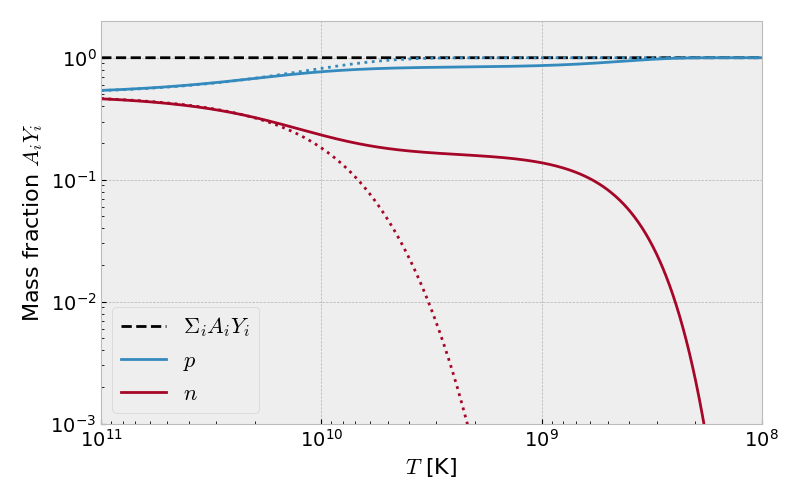
\includegraphics[width=\columnwidth]{densities_f.png}
	\caption{Caption}
	\label{fig:problem_f}
\end{figure}

\section{Problem g)}
From Problem a), we recall that
\begin{align}
	\frac{dn_i}{dt} + 3Hn_i = n_b H \frac{dY_i}{d\ln{T}}
\end{align}
Inserting the given expression
\begin{align}
	\frac{dn_i}{dt} + 3Hn_i
	\ \	=\ \ &\sum\limits_{j\neq i} [n_j\Gamma_{j\rightarrow i} - n_i\Gamma_{i\rightarrow j}] \\
		+ &\sum\limits_{jkl} [n_k n_l\gamma_{kl\rightarrow ij} - n_i n_j\gamma_{ij\rightarrow kl}]
\end{align}
and using the definition $\Gamma_{ij\rightarrow kl} = n_b \gamma_{ij\rightarrow kl}$,
we see that
\begin{align}
		  \frac{dY_i}{d\ln{T}}
		= \frac{1}{H}\bigg\{
		  &\sum\limits_{j\neq i} [\frac{n_j}{n_b}\Gamma_{j\rightarrow i} - \frac{n_i}{n_b}\Gamma_{i\rightarrow j}] \\
		+ &\sum\limits_{jkl} [\frac{n_k}{n_b}\frac{n_l}{n_b} n_b\gamma_{kl\rightarrow ij}
													- \frac{n_i}{n_b}\frac{n_j}{n_b} n_b\gamma_{ij\rightarrow kl}]
			\bigg\} \\
		= \frac{1}{H}\bigg\{
		  &\sum\limits_{j\neq i} [Y_j \Gamma_{j\rightarrow i} - Y_i \Gamma_{i\rightarrow j}] \\
		+ &\sum\limits_{jkl} [Y_k Y_l \Gamma_{kl\rightarrow ij}
													- Y_i Y_j \Gamma_{ij\rightarrow kl}]
			\bigg\}
\end{align}
Which is what we wanted to show.
\section{Problem h)}
Implementing the additional reactions results in Fig. (\ref{fig:problem_h}).
The plot shows a drop in proton and neutron mass fraction as the temperature
decreases past $\sim 10^9$K. This is due to the formation of deuterium, which
has a sharp increase in its mass fraction before it stabilizes at
$A_{D} Y_{D} \sim \frac{1}{4}$ due to exhausting the neutron supply.
\begin{figure}[h]
	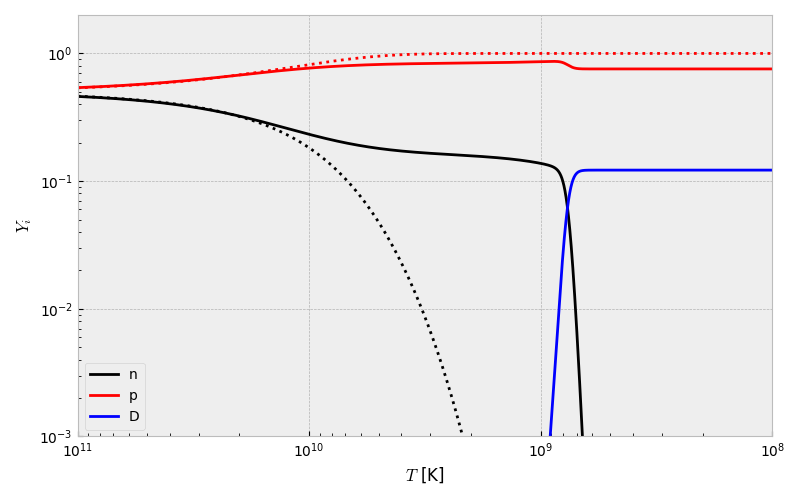
\includegraphics[width=\columnwidth]{densities_h.png}
	\caption{Caption.}
	\label{fig:problem_h}
\end{figure}

\section{Problem i)} \label{ref:task_i)}
Implementing the remaining reactions we get the plot shown in Fig.
(\ref{fig:problem_i}). Ignoring neutrons and protons, the plot shows the
production of most elements happens in the range $\sim 10^{10} - 10^9$ K with
most of the mass fractions peaking at $\sim 10^{9}$K (i.e. $\sim 3$ minutes
after the big bang).
\\ \\
The big exception to this is $Be^7$ which has sharply increases a little bit after
this, while most other elements (an exception being $He^3$) quickly drops in their
mass fractions. This is presumably due to being too large, and possibly requiring
sufficient amounts of other elements to form.
\\ \\
We also note that by the time the temperature has decreased to $10^7$K, the
production of elements seems to have halted completely.
\begin{figure}[h]
	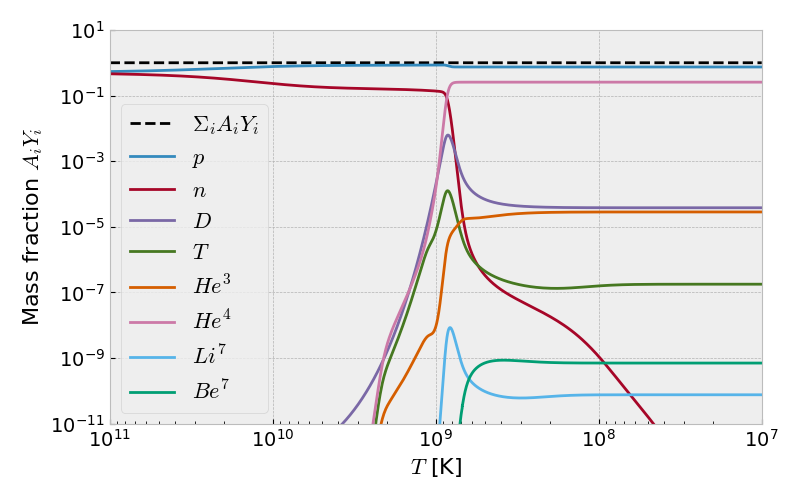
\includegraphics[width=\columnwidth]{densities_i.png}
	\caption{Caption.}
	\label{fig:problem_i}
\end{figure}

\section{Problem j)}
To compute the relic abundances from BBN, we simply pick out the last values
from the simulation in the previous task. In order to find the optimal value for
the baryonic matter content $\Omega_{b0}$, we compute the relic abundances for
$\Omega_{b0}\in[0.01,1]$, and use the chi square method to find the best
fit given the data. This gives an optimal value of $\Omega_{b0}=0.05$. A plot
of the results is attached in Fig. (\ref{fig:problem_j}).
\\ \\
Comparing the results with the total matter content $\Omega_{m0}\approx0.3$,
we see that baryonic matter only makes up around $\Omega_{b0}/\Omega_{m0} = 16.7\%$
of total matter in the universe. Given that most of $\Omega_{m0}$ is in the form
of dark matter, this indicates dark matter is a sort of non-baryonic matter.
For example, one possibility is that dark matter is composed of some unknown
elementary particles.

\begin{figure}[h]
	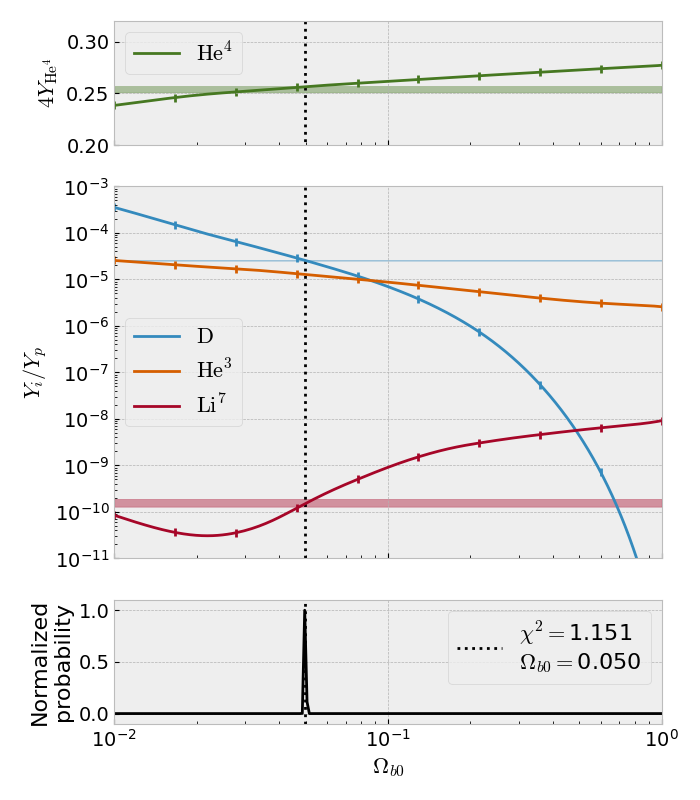
\includegraphics[width=\columnwidth]{relic_abundances_j.png}
	\caption{Relic abundances of elements produced in BBN as function of the baryonic
					matter content $\Omega_{b0}$, as well as the likelihood of different
					$\Omega_{b0}$ given the data. The relic abundances are calculated for
					10 different values of $\Omega_{b0}$ (indicated by notches), which are
					interpolated in order to create smooth functions of $\Omega_{b0}$.}
	\label{fig:problem_j}
\end{figure}

\section{Problem k)}
Computing the relic abundances for $N_{\mathrm{eff}} \in [1, 5]$ we find that
the best fit given the data is $N_{\mathrm{eff}}=3.002$ effective number of
neutrino species (Fig. \ref{fig:problem_k}). This matches well with what we
expect from the standard model, which predicts three neutrino species from its
three generations of elementary particles.
\begin{figure}[h]
	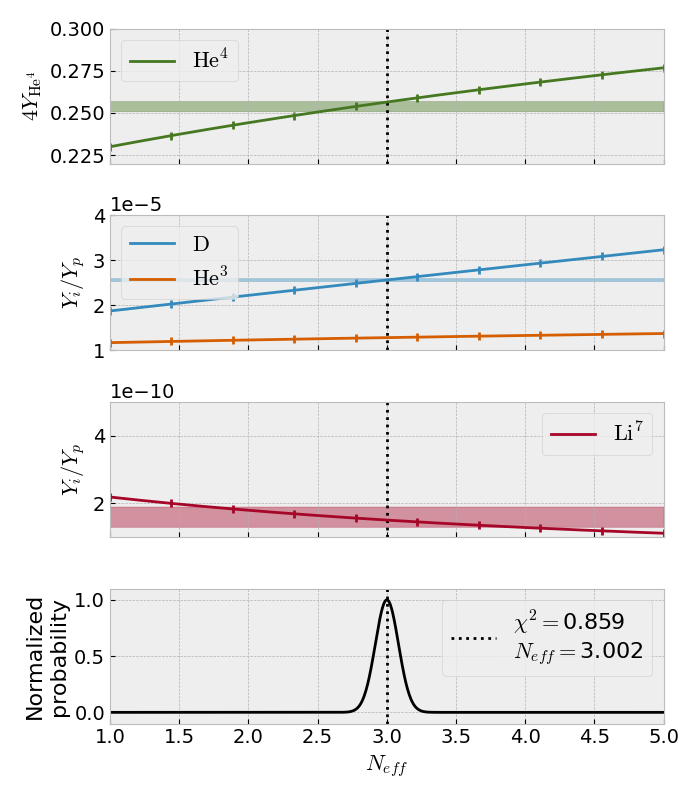
\includegraphics[width=\columnwidth]{relic_abundances_k.png}
	\caption{Relic abundances of elements produced in BBN as function of the
					effective number of neutrino species $N_{\mathrm{eff}}$, and the
					likelihood of different values for $N_{\mathrm{eff}}$ given the data.
					The relic abundances are calculated for 10 different values of
					$N_{\mathrm{eff}}$ (indicated by notches), which are interpolated in
					order to produce smooth functions of $N_{\mathrm{eff}}$.}
	\label{fig:problem_k}
\end{figure}



\begin{acknowledgments}  % if you disagree with the spelling, blame Americans
I would like thank myself for writing this beautiful document.
\end{acknowledgments}

\end{document}
